\documentclass[12pt]{article}	

\usepackage[margin=1in]{geometry}
\usepackage{amsmath,amssymb,amsthm}
\usepackage{graphicx}
\usepackage{caption}
\usepackage{subcaption}
\usepackage{url}
\usepackage{mathrsfs}
\newtheorem{theorem}{Theorem}
\newtheorem{notation}{Notation}
\newtheorem{claim}{Claim}
\newtheorem{lemma}{Lemma}
\newtheorem{definition}{Definition}
\renewcommand{\qedsymbol}{$\blacksquare$}
\newtheorem*{remark}{Remark}

\begin{document}
	\quad \quad \quad \quad \quad \quad \quad \quad \quad \quad  \quad \quad \quad \quad \quad \quad \quad \quad \quad \quad  \quad \quad \quad \quad \quad \quad \quad \quad \quad \quad  Arun Suresh
	\begin{center}
		Homework 4
	\end{center} 
	{\rule{\linewidth}{0.1mm} }
	
\indent $1.$ The Haar function is defined as $H(x) =  \begin{cases} 
0 & x< 0 \\
1 & 0\leq x < \frac{1}{2} \\
-1 & \frac{1}{2} \leq x < 1\\
0 & 1<x 
\end{cases}$\\
Plotted below is the Haar function and a time-shifted version (with a timeshift of $-2$) \\
\begin{figure}[h]
	\centering
	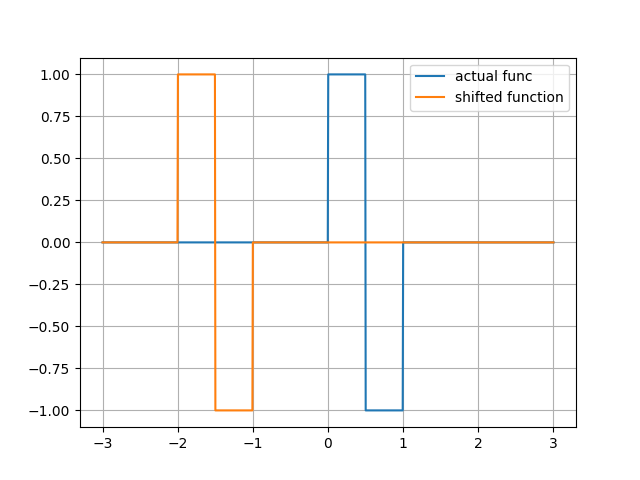
\includegraphics[scale=0.40]{Haar_space_domain.png}
	\caption{Plots of original and timeshifted Haar function}
\end{figure}

The fourier transform of the Haar function was calculated in Python (ver 3.70) using two different numerical packages. The first one was the FFT functionalities that come included with the numpy library for python. The second one was the pyFFTW, which is the python wrapping of regular FFTW method written for C++. A mask was applied to filter out all the negative frequencies that are symmetric to the positive frequency side (This comes  as a part of both FFTW and Numpy.fft, as a normalization method so that the inverse fourier transform could be computed with relative ease) \\ 
The following are the plots of the fourier transform using the numpy fft functionalities.
\begin{figure}[h]
	\centering
	\begin{subfigure}[h]{0.40\textwidth}
		\centering
			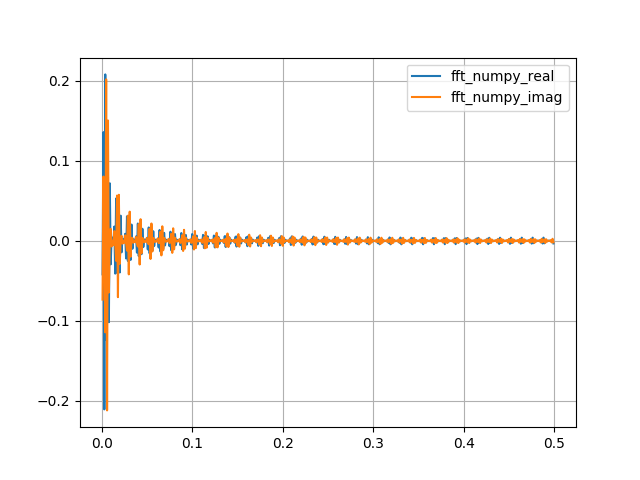
\includegraphics[width=\textwidth]{freq_domain_numpy_full.png}
		\caption{full FT}
	\end{subfigure}
	\begin{subfigure}[h]{0.40\textwidth}
		\centering
			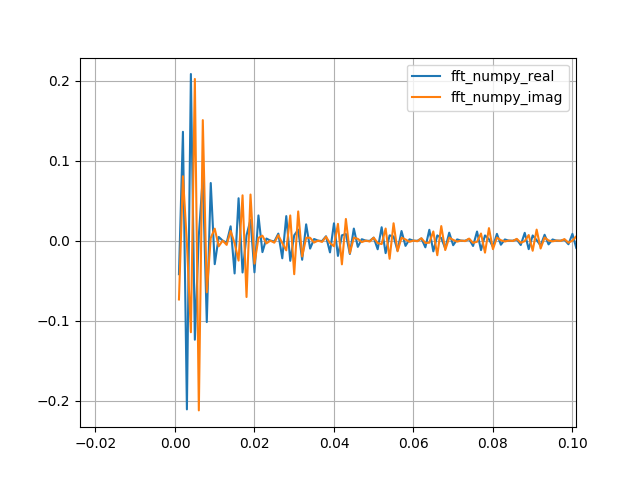
\includegraphics[width=\textwidth]{freq_domain_numpy_nonshift.png}
		\caption{FT zoomed}
	\end{subfigure}
	\caption{Numpy FFT}
\end{figure}
\\\\\\
The following are the plots of the fourier transform using the pyFFTW library.
\begin{figure}[h]
	\centering
	\begin{subfigure}[h]{0.40\textwidth}
		\centering
		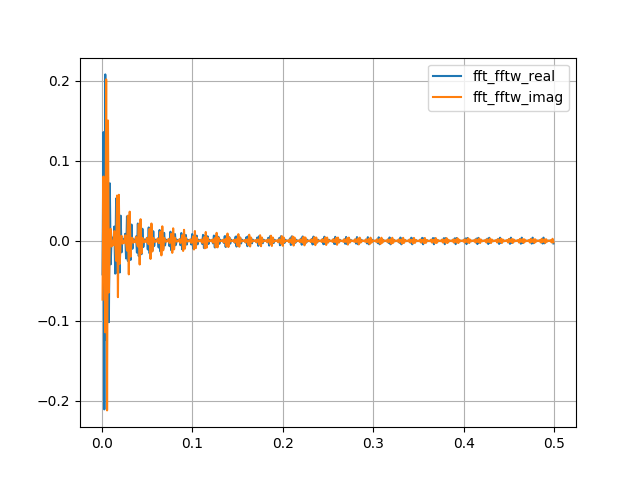
\includegraphics[width=\textwidth]{freq_domain_fftw.png}
		\caption{full FT}
	\end{subfigure}
	\begin{subfigure}[h]{0.40\textwidth}
		\centering
		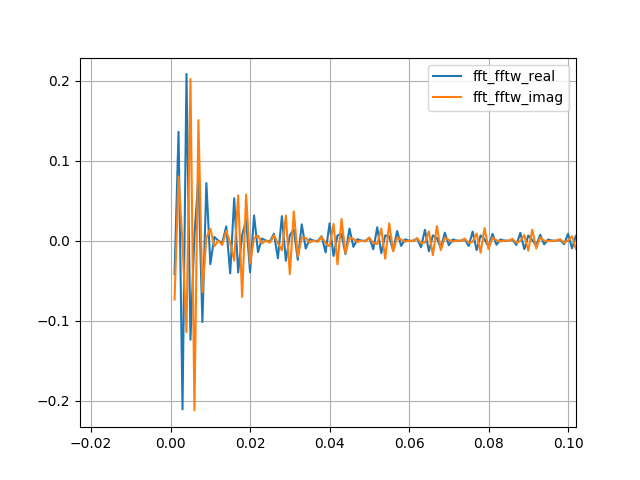
\includegraphics[width=\textwidth]{freq_domain_fftw-zoom.png}
		\caption{FT zoomed}
	\end{subfigure}
	\caption{FFTW}
\end{figure}

The y-axis for the above plots, and for all plots that follow measures the amplitude of each constituent wave, while the x-axis measures the scaled\footnote{actual frequency can be obtained by computing $(x-value)*\frac{N}{6}$ where $N=1000$ is the number of frequency samples and $6$ is the length of the axis $(-3,3)$} frequency of the constituent wave. \\
\indent It is expected that we notice numerous frequencies dying out as $N$ gets larger, because the Haar function is a discontinuous function and thus does not admit a finite fourier series. \\\\

It is more or less clear that both numpy FFT and FFTW both return very similar fourier transforms.  However, the main difference between using Numpy FFT and FFTW is that of computational time. While the numpy FFT took $0.003s$ to complete, FFTW took 7.886$\times10^{-5}s$ to finish, which is considerably faster than numpyFFT, considering that this was performed only over a thousand data points. Presented below is a screenshot of the compilation time printed to the console. 
\begin{figure}[h]
	\centering
	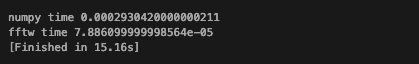
\includegraphics[scale=0.40]{timediff.png}
	\caption{Computation time}
\end{figure}

The fourier transforms of the timeshifted Haar function were also computed and plotted alongside the fourier transforms of the non-timeshifted Haar function. The plots are presented below.
\begin{figure}[h]
	\centering
	\begin{subfigure}[h]{0.40\textwidth}
		\centering
		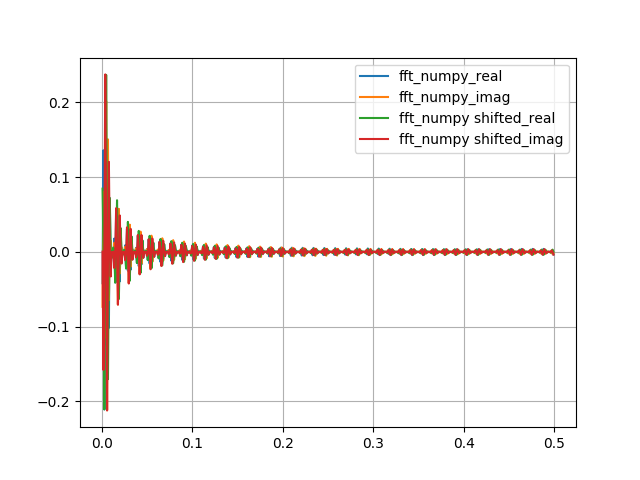
\includegraphics[width=\textwidth]{freq_domain_numpy_final_nozoom.png}
		\caption{full FT}
	\end{subfigure}
	\begin{subfigure}[h]{0.40\textwidth}
		\centering
		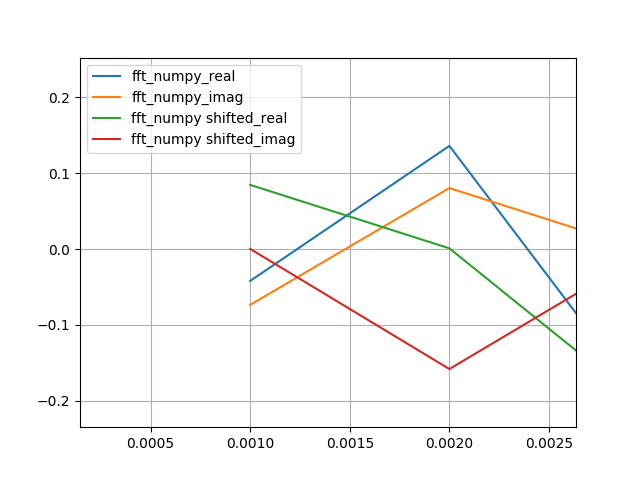
\includegraphics[width=\textwidth]{freq_domain_numpy_final_zoom.png}
		\caption{FT zoomed}
	\end{subfigure}
	\caption{Numpy FFT zero vs. non-zero timeshift}
\end{figure}
\\\\\\\\ Initially looking at the non-zoomed fourier transform, it looks like a cacophonous mess of plots. So, we zoom into just one of the spikes to analyze what is really happening.  In figure 5(b), it is abundantly clear what is happening. Notice that a timeshift to the space domain, produces a complex phase factor in the frequency domain - this means that the original solution is just rotated by some angle in the complex plane. This in turn means, that the real and imaginary values of the output oscillate in such a way that the magnitude is preserved (as the magnitude of any phase factor is 1). \\ Looking at plot 5(b), we can observe this happening. Notice that the real and imaginary part of the non-shifted FT are different from the ones of the shifted ones. However, both of their magnitudes are the same $\sqrt{0.08^2 + 0.136^2} \approx \sqrt{0^2 + 0.157^2} \approx 0.157$. This fact is even more clear when we plot out the absolute value (which coincides for timeshift and non-timeshift version of the function) of our complex output instead of real and imaginary parts seperately. Presented below is that plot. 

\begin{figure}[h]
	\centering
	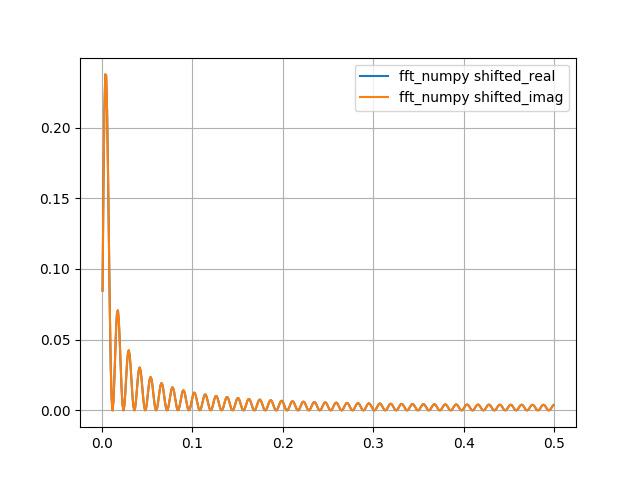
\includegraphics[scale=0.40]{magnitudes.png}
	\caption{Magnitudes}
\end{figure}

Results from FFTW and Numpy.fft once again coincided just like before. The above plots are only those obtained from numpy.fft and the FFTW plots are not provided to reduce redundancy. The time difference in computation was once again significant, with FFTW performing much better than numpy.fft 
\newpage 
$2.$ The Sine cardinal function is given by $F(k)= \begin{cases}
1 & k=0 \\
\frac{\sin(k)}{k} & otherwise
\end{cases}$
Plotted below is the Sine cardinal function and a time-scaled version of it (by a factor of 2).
Notice that in this case, the function is already given in the frequency domain, and we are required to calculate the inverse fourier transform. 
\begin{figure}[h]
	\centering
	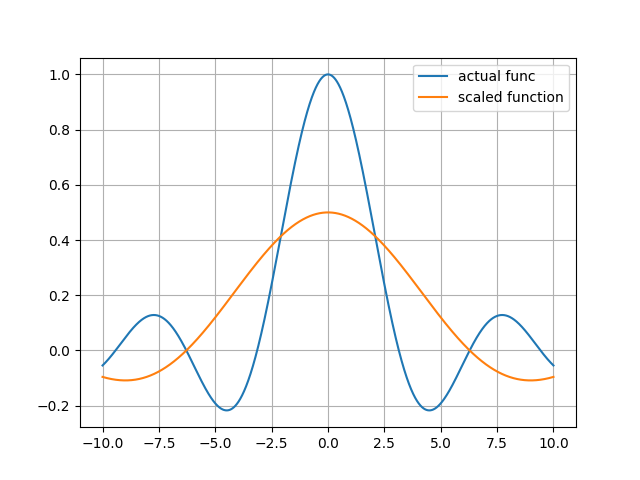
\includegraphics[scale=0.40]{2/space_domain-sinecardinal.png}
	\caption{Sine cardinal function in the Frequency domain}
\end{figure}

The x-axis represents frequency and the y-axis represents the amplitudes. The inverse fourier transform was calculated using the same two packages used in the previous problem. A mask was once again applied to filter out all the negative space values (which would be symmetric) The corresponding IFT plots for the non-scaled and time-scaled functions are presented in Figures 8 and 9. The absolute value of the output was calculated for the plots (this was done to avoid a few numerical errors that might have been occurred)\footnote{Since the sine cardinal function is an even function, we expect the imaginary part of the output to be $0$ always. However, upon plotting the real and imaginary parts, some noise was observed in both outputs. In order to rectify that error completely, the absolute value was computed}
\begin{figure}[h]
	\centering
	\begin{subfigure}[h]{0.40\textwidth}
		\centering
		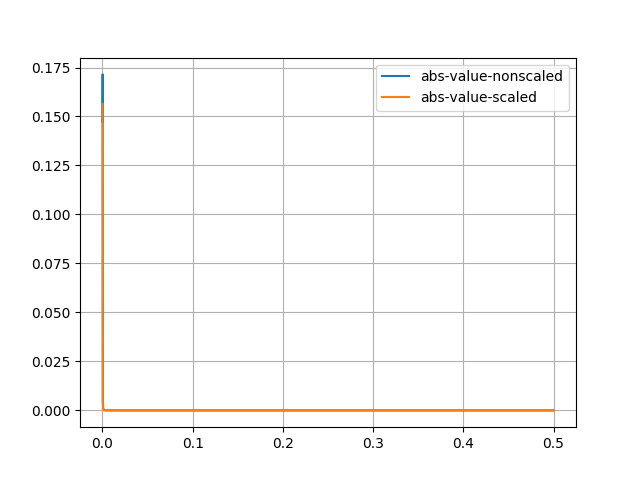
\includegraphics[width=\textwidth]{2/freq_domain_absolute_value_-_np-fft-sinecardinal.png}
		\caption{full FT}
	\end{subfigure}
	\begin{subfigure}[h]{0.40\textwidth}
		\centering
		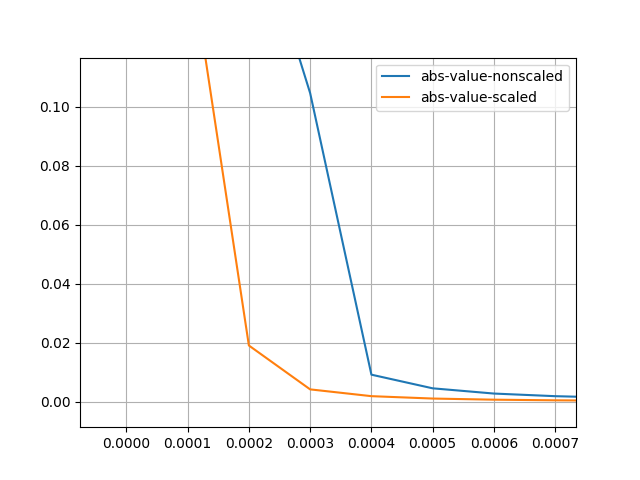
\includegraphics[width=\textwidth]{2/freq_domain_absolute_value_-_np-fft-sinecardinalzoom.png}
		\caption{FT zoomed}
	\end{subfigure}
	\caption{Numpy FFT}
	\centering
	\begin{subfigure}[h]{0.40\textwidth}
		\centering
		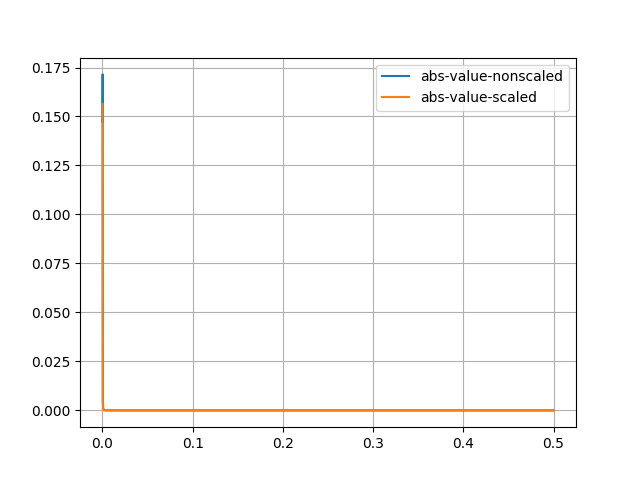
\includegraphics[width=\textwidth]{2/freq_domain_absolute_value_-_fftw-sinecardinal.png}
		\caption{full FT}
	\end{subfigure}
	\begin{subfigure}[h]{0.40\textwidth}
		\centering
		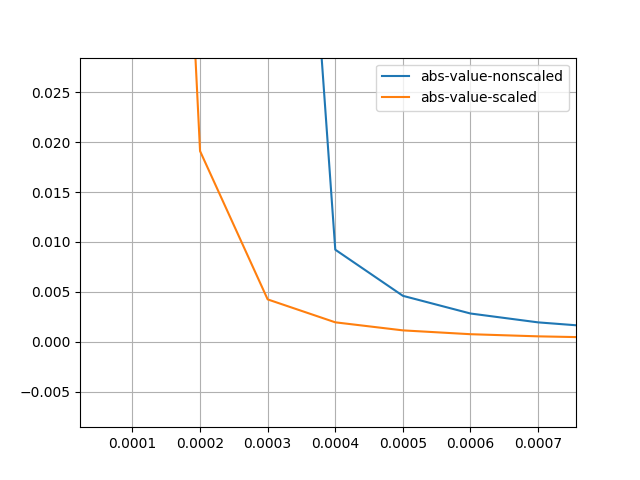
\includegraphics[width=\textwidth]{2/freq_domain_absolute_value_-_fftw-sinecardinalzoom.png}
		\caption{FT zoomed}
	\end{subfigure}
	\caption{FFTW}
\end{figure}
\\\\ It is apparent that both numpy.fft and FFTW returned very similar looking plots (although, it seems as it FFTW had a little bit of a better smoothing than numpy.fft and we had to zoom in considerably to notice the linear numerical approximation of the curve). The time difference in computation was once again significant with FFTW performing far better than numpy.fft - by a factor of 100. Presented in Figure 10 is the time data that was output to the console.\footnote{due to some Latex issue, I was not able to typeset the images to their proper spots} The fftw performed to its fullest efficiency during its second computation compared to the first, because it is possible that a significant amount of time was spent in loading up the module during its first computation. \\\\
\begin{figure}[h]
	\centering
	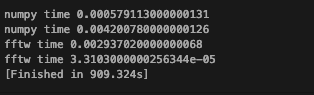
\includegraphics[scale=0.40]{2/timediff.png}
	\caption{Time differences in computation}
\end{figure}
The time scaling is also very apprent in the zoomed version of the plots in Figure 8 and 9. We notice that the scaled function is shrunk by a factor of $2$, which is what we would expect from a timescaling by a factor of $2$. 


\end{document}